\documentclass[11pt]{article}

% Language setting
\usepackage[english]{babel}

% Set page size and margins
\usepackage[a4paper,top=2cm,bottom=2cm,left=3cm,right=3cm,marginparwidth=1.75cm]{geometry}

% Packages
\usepackage{amsmath}
\usepackage{amsfonts}
\usepackage{amsthm}
\usepackage{graphicx}
\usepackage{enumerate}
\usepackage[hidelinks]{hyperref}
\graphicspath{ {./images/} }
\bibliographystyle{abbrv}
\theoremstyle{definition}
\newtheorem{exmp}{Example}[section]
\newtheorem{definition}{Definition}[section]

\hypersetup{
    colorlinks=false,
    linkcolor=blue,
    filecolor=magenta,      
    urlcolor=cyan,
    pdftitle={Overleaf Example},
    pdfpagemode=FullScreen,
    }

\title{Chaos in Discrete Dynamical Systems}
\author{Fraser Love}

\begin{document}
\maketitle

\noindent\textit{I certify that this project report has been written by me, is a record of work carried out by me, and is essentially different from work undertaken for any other purpose or assessment.}

\vspace{0.1cm}\hspace{13.1cm}
\includegraphics[width=1.3cm]{signature}

\begin{abstract}
    \noindent This project explores the wonders of chaotic discrete deterministic dynamical systems through the lense of pure Mathematics. We will define the many notions of chaos in a dynamical system and explore numerous examples of chaotic discrete systems and aim to understand their natural beauty. The mathematics in this paper is aimed at an interested undergraduate student with a solid understanding of calculus and real analysis.
\end{abstract}

\tableofcontents

\section{Introduction}
\subsection{Dynamical Systems}
A dynamical system is a set of states governed by a rule which specifies how the states evolve over time. Dynamical systems can either be discrete or continuous throughout time. A continuous dynamical system is described by a differential equation of any form (e.g. $dx/dt = F(x)$, where $F: X \to X$ is some function). In this project however, we will be focusing on examining discrete dynamical systems only. Moreover all the dynamical systems will be deterministic (i.e. discrete systems where the present state is uniquely determined by previous states). \cite{devaney} \cite{ruette} \cite{asy} \cite{cobweb}

\begin{definition}
    Let $X$ be a set. A discrete dynamical system is given by a map $f : X \to X$. The system starts at a point $x$ and evolves through iterative applications of the map $f$ on points in $X$. After $n$ iterations of $f$ the system can be described by $f^n(x) = f \circ f \circ \cdots \circ f(x)$ where $n \in \mathbb{N}$. Any point $x_n$ can be described by the transformation of $f$ on its previous state as follows: $x_n = f(x_{n-1})$. 
\end{definition}

\begin{exmp}
The simplest discrete dynamical system could be the doubling map: \[f : \mathbb{R} \to \mathbb{R}, x \mapsto 2x\] Where each new state can be calculated from the previous state as follows: \[x_n = 2x_{n-1}\] Let $x_0$ be the initial value of the system. The value of the system after $n$ iterations of the map $f$ is given by: \[x_1 = f(x_0) = 2x_0\] \[x_2 = f(x_1) = f^2(x_0) = f^2(x_0) = 4x_0\] \[\vdots\] \[x_n = f(x_{n-1}) = f^2(x_{n-2}) = \cdots = f^n(x_0) = 2^nx_0\] This dynamical system grows exponentially and is unbounded.
\end{exmp}

\begin{exmp}
    A more interesting example is the logistic map $g: [0,1] \to [0,1]$ where $g(x)=rx(1-x)$. Lets initially set $r = 2$. Hence we have the discrete system: \[x_n = g(x_{n-1}) = 2x_{n-1}(1 - x_{n-1})\] For $x \ll 1$, $g(x) \simeq 2x$, however for $x \gg 0$, $g(x) \simeq 2(1-x) < 1$. It will be shown later that any initial $x_0 \neq 0, 1$ will be attracted towards the fixed point of $x = 1/2$. The logistic map is integral to discrete dynamical systems and we shall examine it alot more further into the project.
\end{exmp}

\begin{definition}
    Let $f: X \to f(X)$ be a map and $x \in X$. The orbit of $x$ under $f$ is the set \[\mathcal{O}_f(x) = \lbrace f^n(x) : n \geq 0 \rbrace = \lbrace x, f(x), f^2(x), \cdots \rbrace\] of iterates of $x$ under $f$.
\end{definition}

\begin{definition}
    The trajectory of $x$ is the infinite sequence $(f^n(x))_{n \geq 0}$. If $x$ is periodic there will be repetitions in this sequence.
\end{definition}

\begin{definition}
    A periodic point is a point $x \in X$ such that $f^n(x) = x$ for some $n \in \mathbb{N}$. Hence, the period of a point $x$ is the least positive integer $p$ such that $f^p(x) = x$. Moreover $f^n(x) = x \iff n = kp$ for some $k \in \mathbb{N}$ (i.e. $n$ is a multiple of $p$). This means that $\mathcal{O}_f(x) = \lbrace x, f(x), \cdots, f^{p-1}(x) \rbrace$ is a finite set of unique points.
\end{definition}

\begin{definition}
    A fixed point is simply a periodic point of period one, so $f(x) = x$. Hence $\mathcal{O}_f(x) = \lbrace x \rbrace$. The fixed points of a system can be simply calculated by setting $f(x) = 0$ and solving for $x$.
\end{definition}

\begin{exmp}
Find the fixed points of the logistic map: \[g(x) = 2x(1-x) = 2x - 2x^2 = 0\] Hence, $x = 0$ and $x = 1/2$ are fixed points, which is true as $g(\frac{1}{2}) = 2 \cdot \frac{1}{2} \cdot (1 - \frac{1}{2}) = \frac{1}{2}$ and $g(0) = 2 \cdot 0 \cdot (1 - 0) = 0$.
\end{exmp}

\subsubsection{Cobweb Plots}
A cobweb plot can be used to explore the long-term stability of the orbit of a 1D map. The sucessive iterates of a map $f$ are plotted on the graph of $f$ and $y = x$, with horizontal and vertical lines used to track the evolution of the system. To constuct a cobweb plot first plot the curves $y = f(x)$ and $y = x$. Then for $n$ sucessive iterations of the map $f$, draw:
\begin{enumerate}[i.]
    \item An initial vertical line from $(x_0, 0)$ to $(x_0, f(x_0))$
    \item Horizontal lines from $(f^i(x_0), f^{i+1}(x_0))$ to $(f^{i+1}(x_0), f^{i+1}(x_0))$ for $0 \leq i \leq n$
    \item Vertical lines from $(f^i(x_0), f^i(x_0))$ to $(f^i(x_0), f^{i+1}(x_0))$ for $1 \leq i \leq n$
\end{enumerate}
\begin{exmp} Cobweb diagrams of the logistic map:
    \begin{figure}[h]
        \centering
        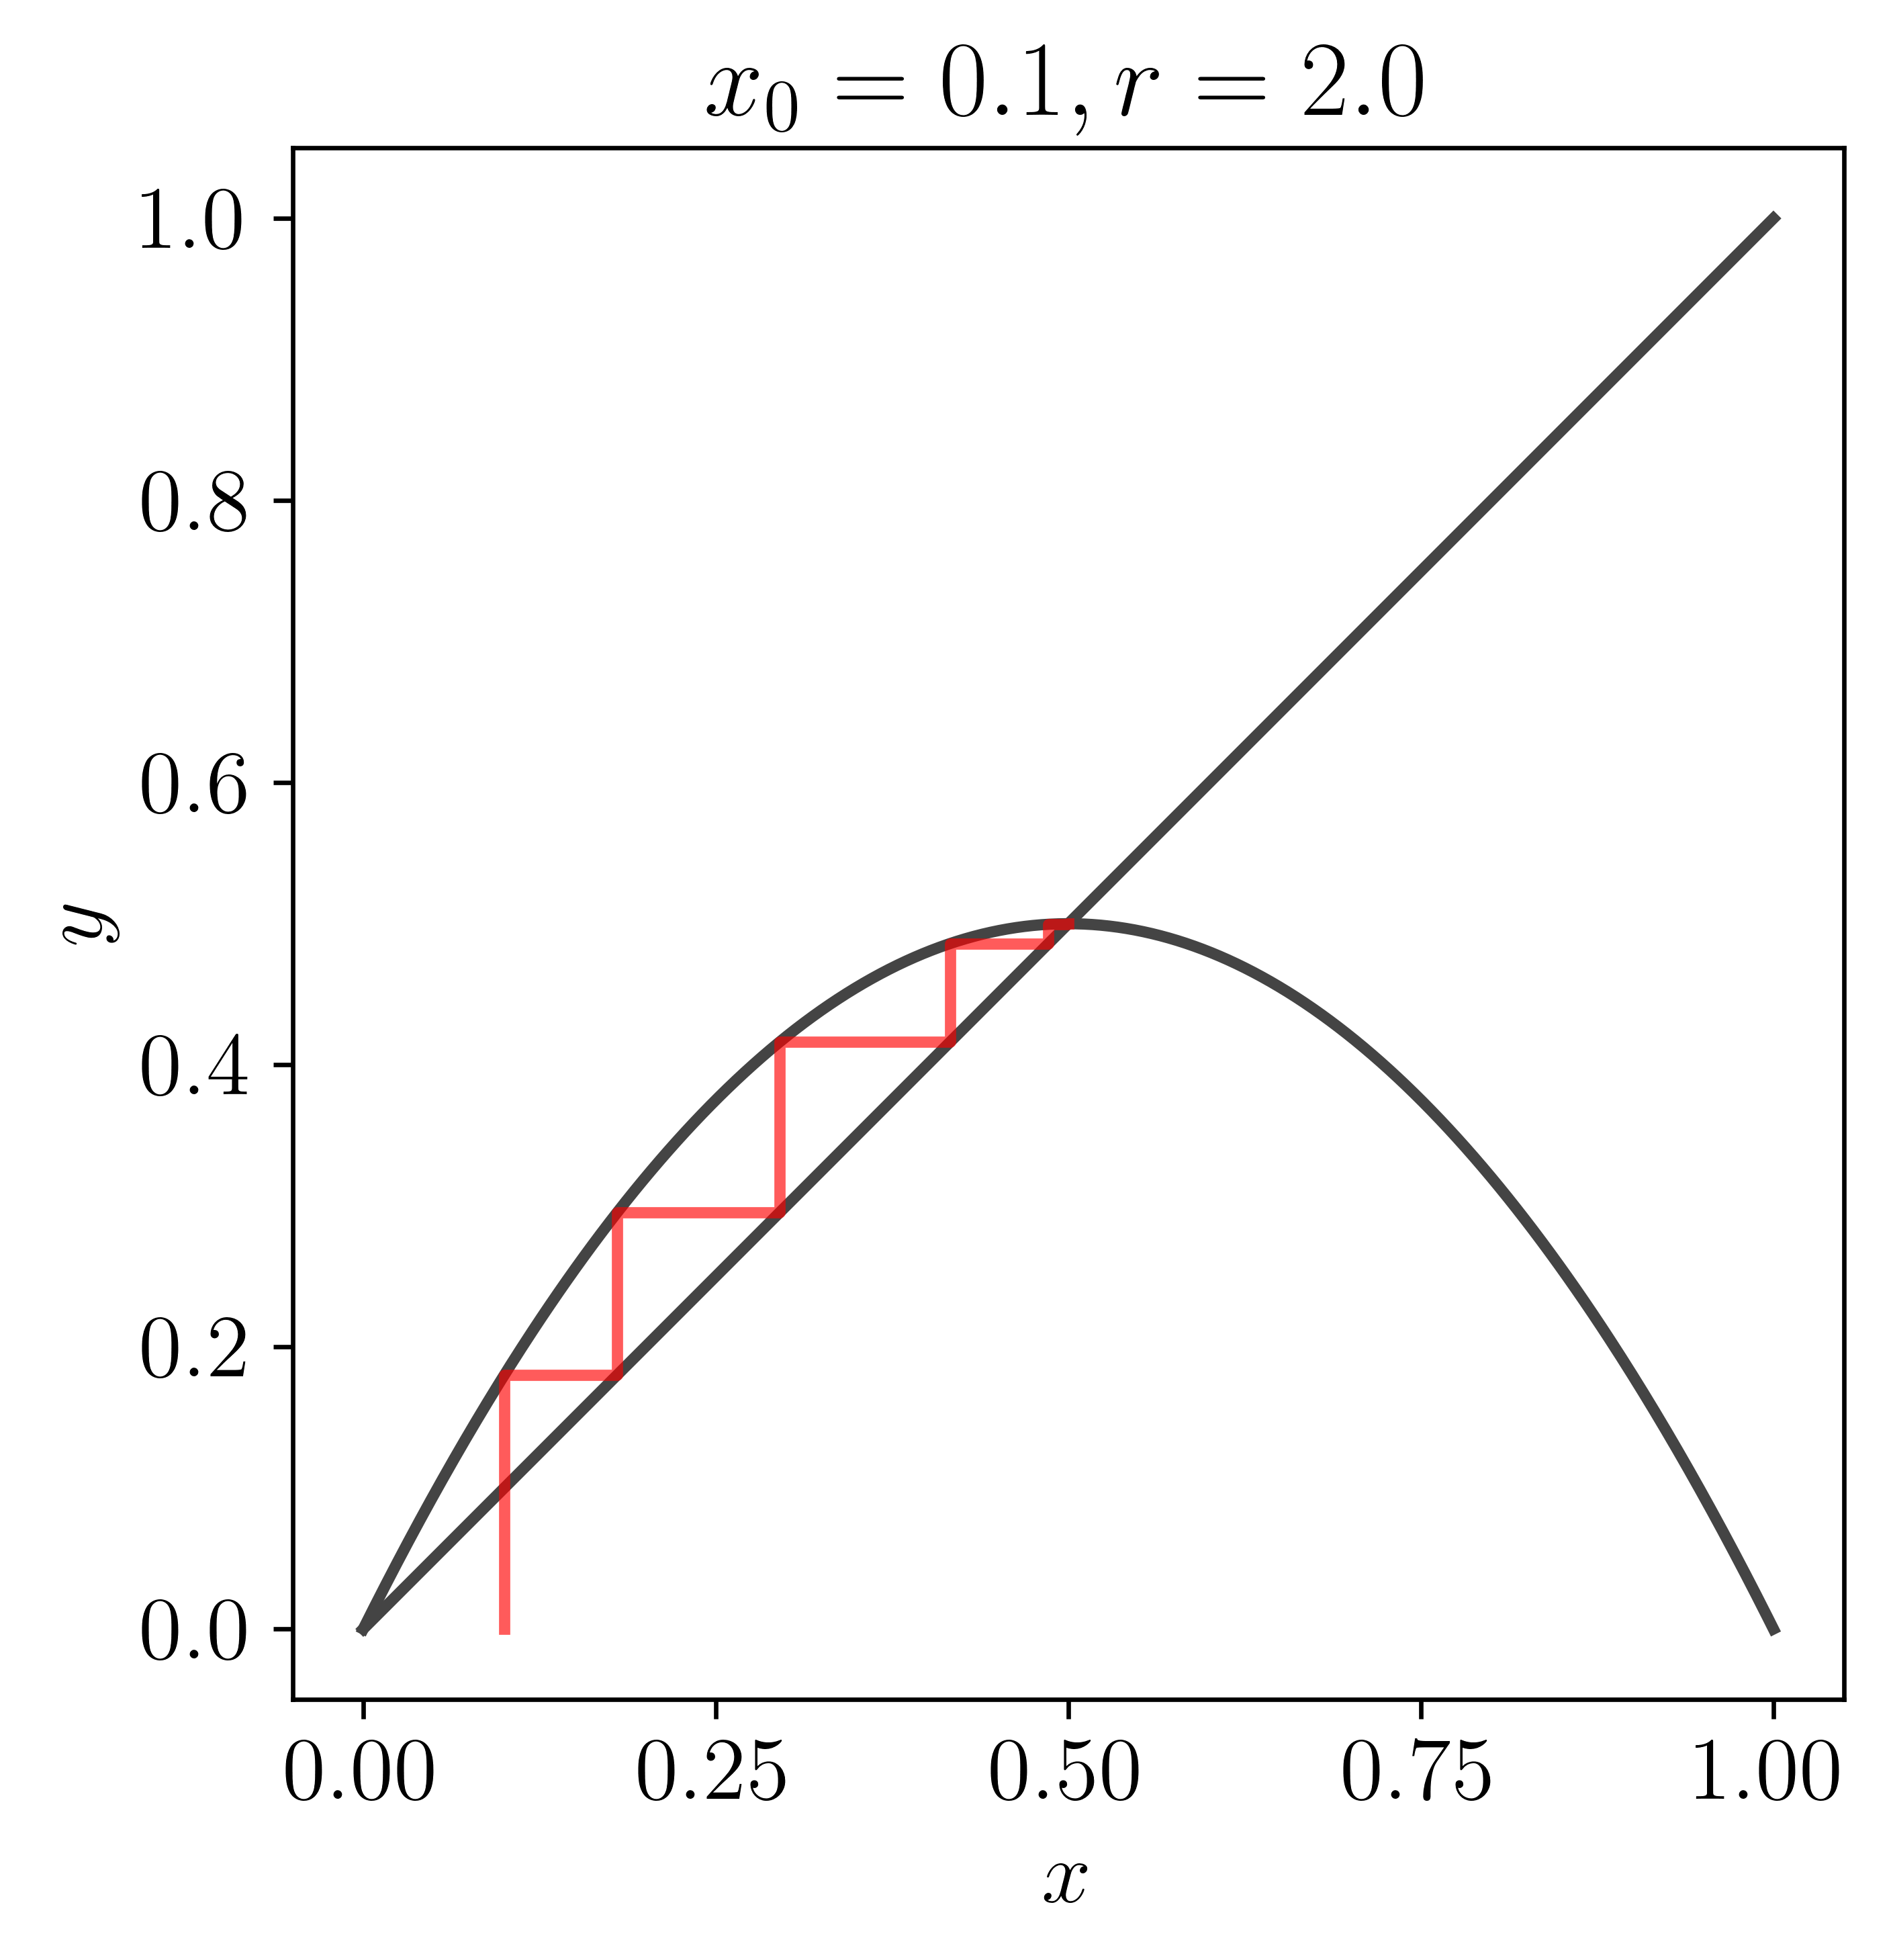
\includegraphics[width=4.9cm]{cobweb_0.1_2.0}
        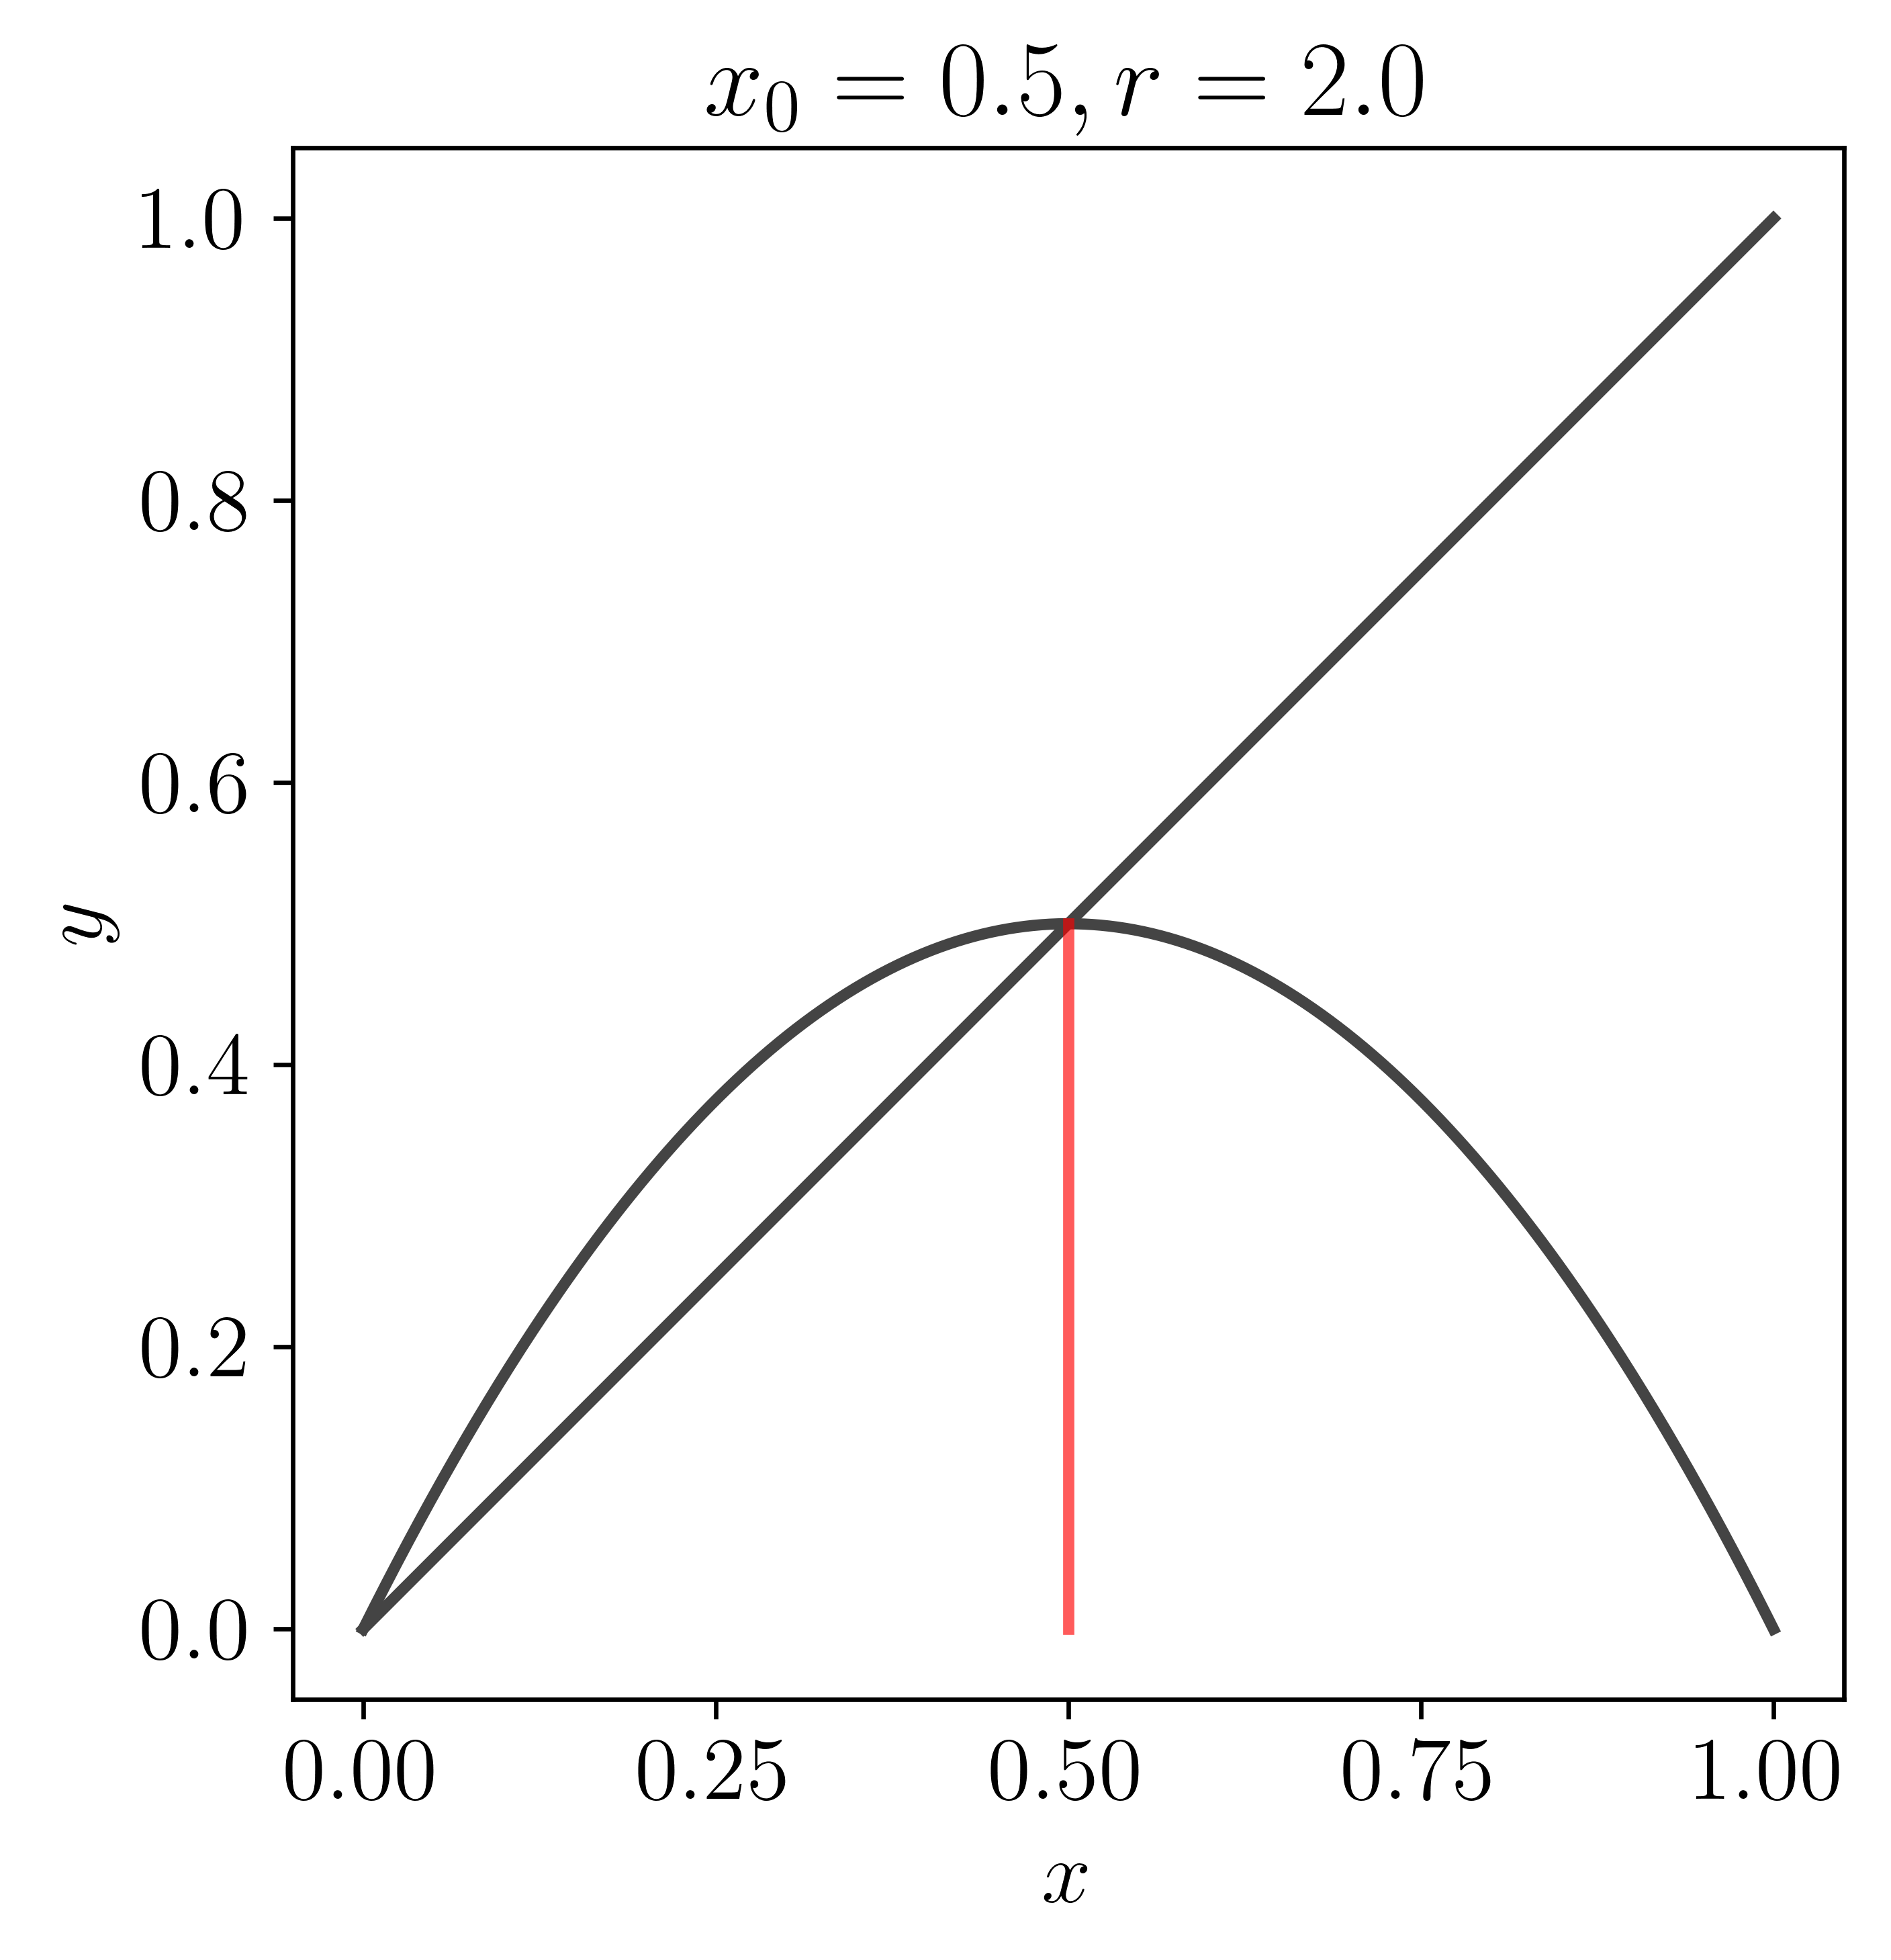
\includegraphics[width=4.9cm]{cobweb_0.5_2.0}
        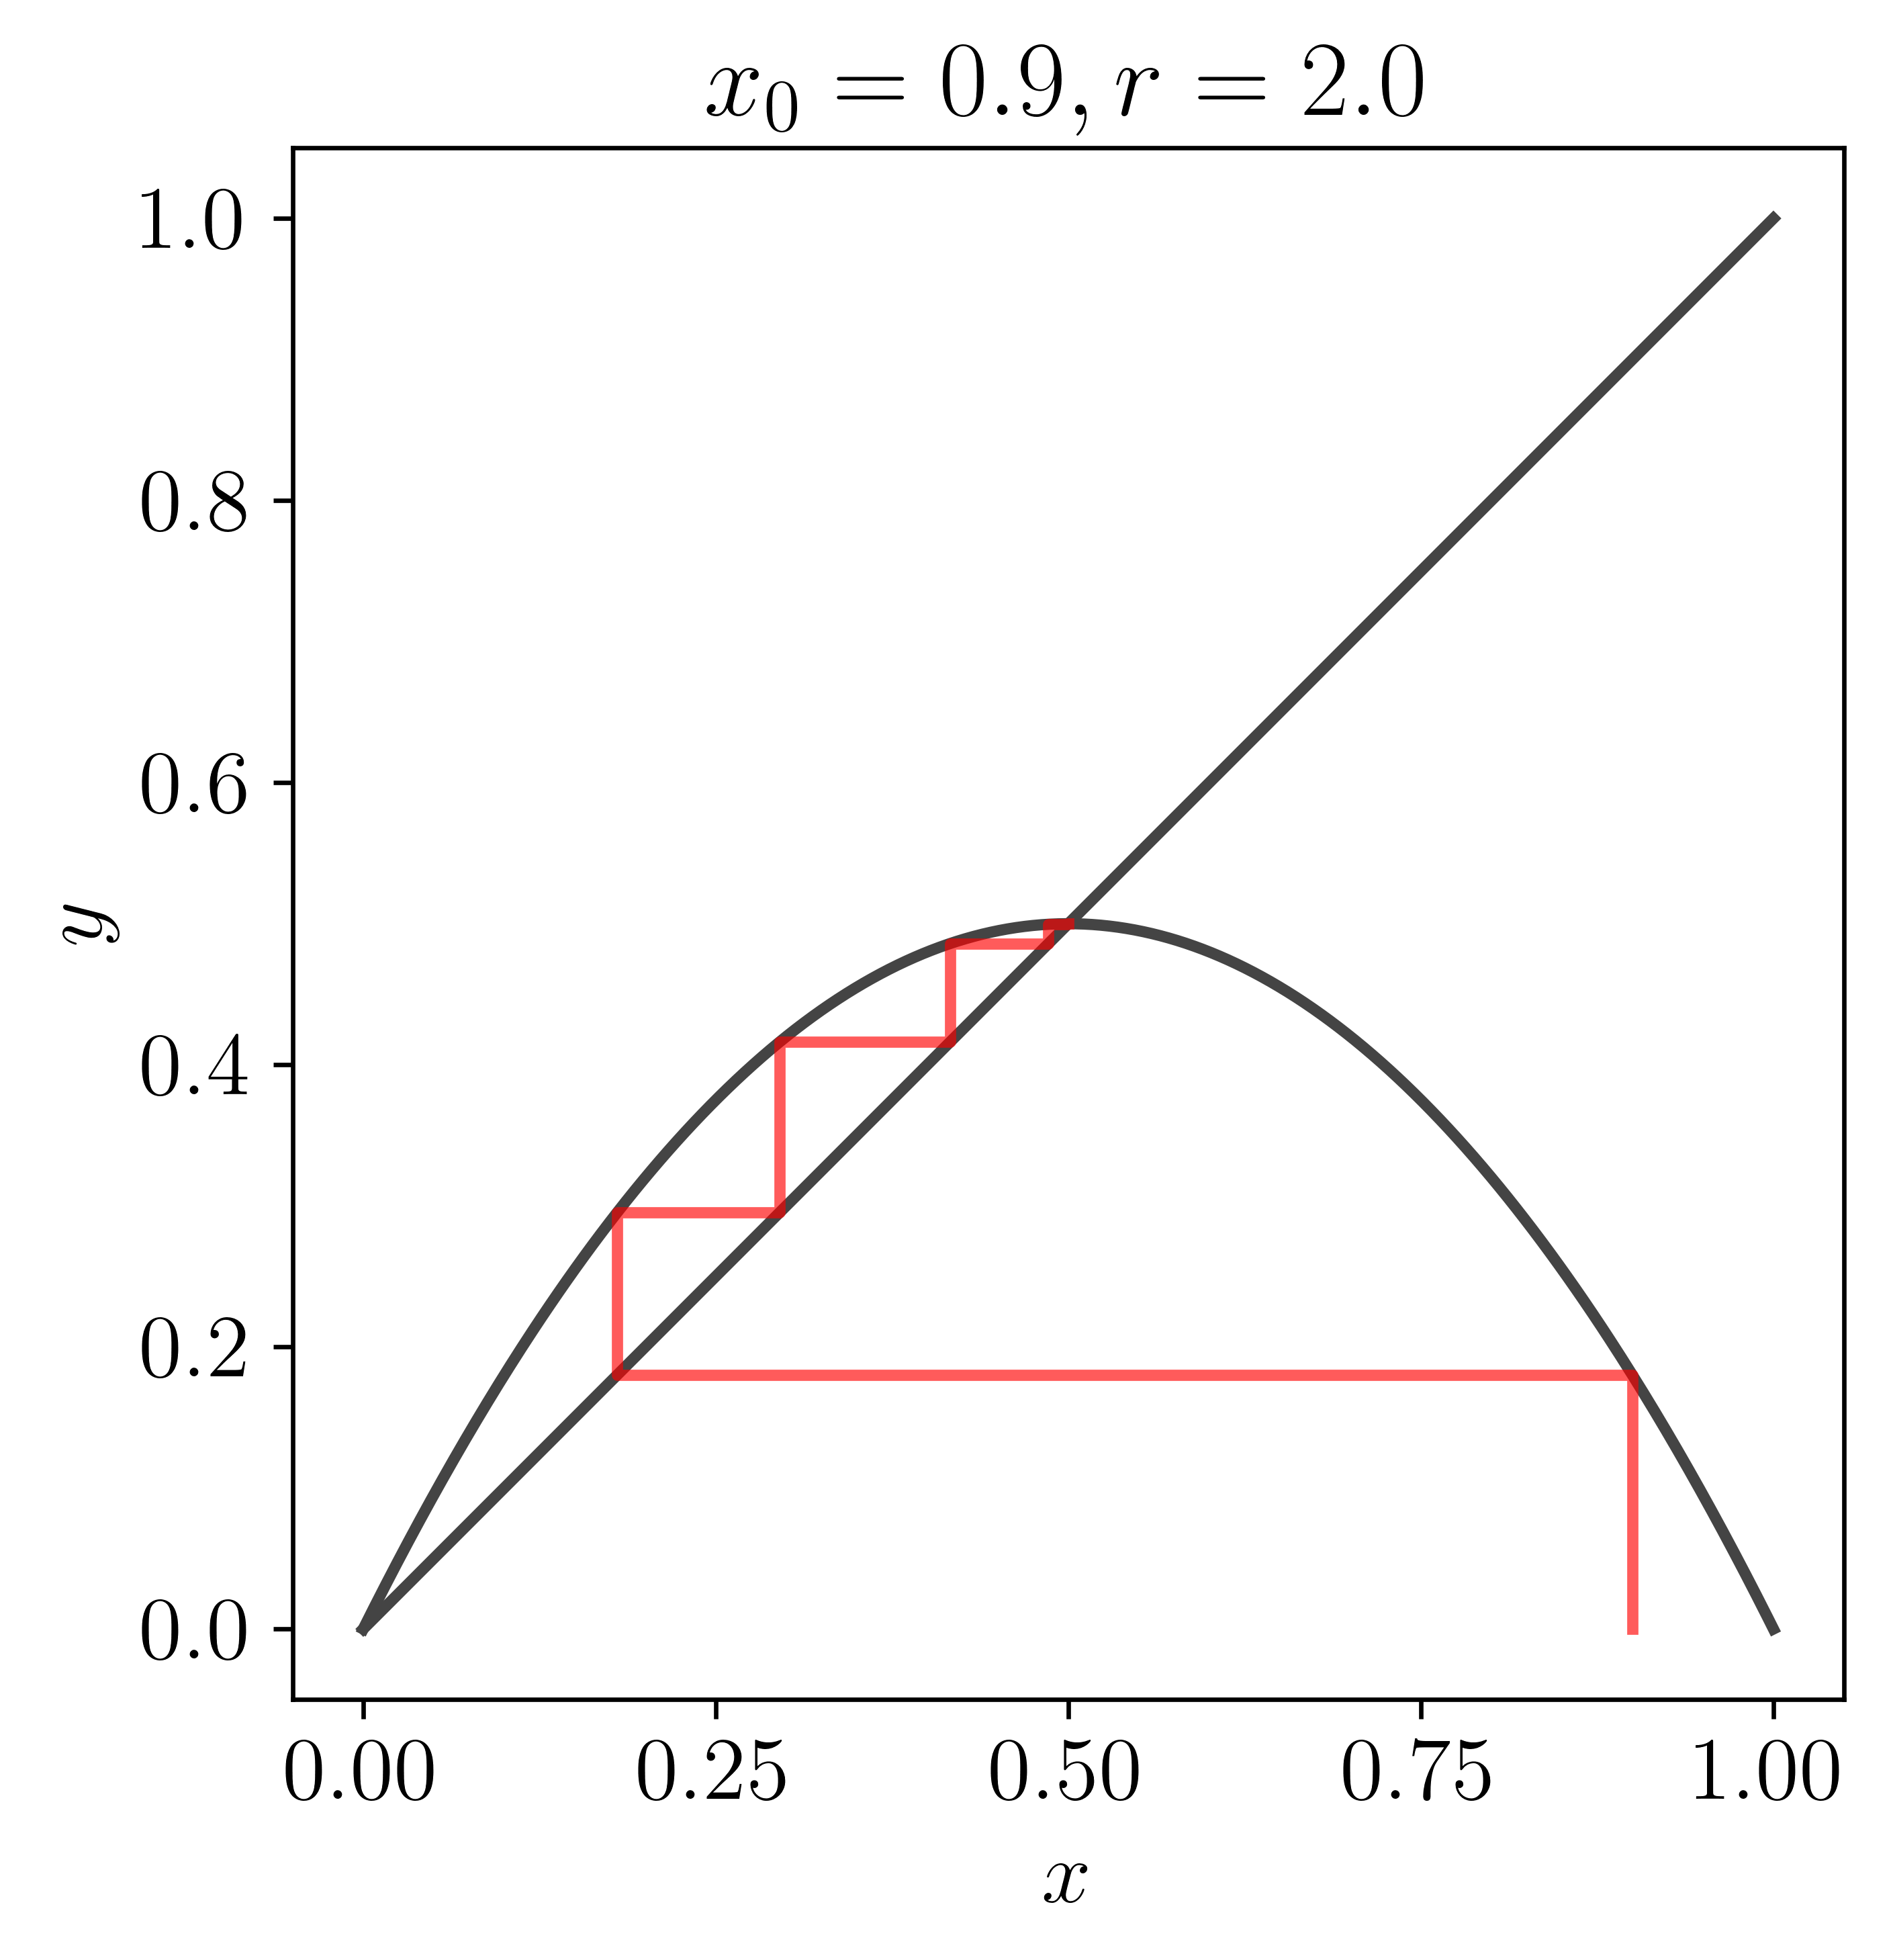
\includegraphics[width=4.9cm]{cobweb_0.9_2.0}
        \caption{Cobweb diagrams of the function $f(x) = 2x(1-x)$ over $40$ iterations with initial values $x_0 = 0.1$, $0.5$ and $0.9$.}
    \end{figure}
    \\
    These cobweb diagrams suggest that no matter what $x_0$ we choose, the dynamical system described by $f(x) = 2x(1-x)$ will spiral in towards the fixed point $x = 1/2$. This is infact the case, to see why we need to define the notion of stability in a dynamical system.
\end{exmp}
\subsection{Stability of Fixed Points}
\begin{definition}
    Hello
\end{definition}
\section{One-Dimensional Maps}
\subsection{Fixed and Periodic Points}
\subsection{Stability of Fixed Points}
\subsection{Logistic Maps}
\section{What is Chaos?}
Brief overview into definitions of chaos with examples.
\section{Periodic Points and Stability}
\section{Higher-Dimensional Dynamical Systems}
\section{Higher-Dimensional Stability}
\section{Chaos in Higher Dimensions}
\subsection{Chaotic Attractors}
\section{Fractals}
\subsection{Julia Sets}

\bibliography{chaos}

\end{document}